% --- Definição da Classe do Documento ---
\documentclass[conference,harvard,brazil,english]{sbatex}

% --- Codificação e Fontes (Correção Essencial) ---
\usepackage[utf8]{inputenc}
\usepackage[T1]{fontenc}
\usepackage{lmodern}

% --- Pacotes Recomendados para Qualidade e Funcionalidade ---
\usepackage{graphicx}   % Para incluir figuras
\usepackage{amsmath}    % Para equações avançadas (já estava no seu código)
\usepackage{amssymb}    % Complementa o amsmath com mais símbolos
\usepackage{booktabs}   % Para tabelas com visual profissional
\usepackage{microtype}  % Melhora o espaçamento e a justificação do texto
\usepackage[hyphens]{url} % Para formatar URLs de forma inteligente
\usepackage{hyperref}   % Cria links clicáveis (citações, seções, etc.) - DEVE SER O ÚLTIMO PACOTE!
\usepackage{float}
% --- Comandos específicos do template original (se necessário) ---
% Estes comandos são necessários apenas para a geração deste artigo exemplo. 
% Eles não fazem parte do estilo SBATeX.
\makeatletter
\def\verbatim@font{\normalfont\ttfamily\footnotesize}
\makeatother

% --- Início do Documento ---
\begin{document}

% O restante do seu código continua aqui...

% CABEÇALHOS

\title{Módulo 1 - Processo Massa Mola}

%%%%%%%%%%%%%%%%%%%%%%%%%%%%%%%%%%%%%%%%%%%%%%%%%%%%%%%%%%%%%
%
% O processo de revisao do CBA 2014 sera DOUBLE BLIND, portanto NAO inclua
% autores na versão que será submetida para revisão
%
%%%%%%%%%%%%%%%%%%%%%%%%%%%%%%%%%%%%%%%%%%%%%%%%%%%%%%%%%%%%%

\author{Eduardo Rodrigues Cordeiro}{eduardorc14@ufmg.br}
\author{Pedro Henrique de Menezes Cosme}{pedrocosme@ufmg.br}

\twocolumn[

\maketitle

\selectlanguage{english}
\begin{abstract}
This work details the mathematical modeling of the ECP Model 210 mass-spring system to obtain a fourth-order model. Physical parameters of mass ($m$), spring constant ($k$), and damping ($b$) were experimentally identified through open-loop tests (step and free response) on simplified configurations. From the data, intermediate second-order models were estimated, which provided the basis for calculating the physical parameters. The final model, expressed in transfer functions, was validated by comparing its simulated response with experimental data, showing good agreement.  \end{abstract}

\keywords{Control Systems, Mass-spring, Position Control, Mathematical Model.}

\selectlanguage{brazil}
\begin{abstract}
Este trabalho detalha a modelagem matemática do sistema massa-mola ECP Model 210 para obter um modelo de quarta ordem. Parâmetros físicos de massa ($m$), constante elástica ($k$) e amortecimento ($b$) foram identificados experimentalmente através de ensaios em malha aberta (resposta ao degrau e livre) em configurações simplificadas. A partir dos dados, foram estimados modelos intermediários de segunda ordem, que serviram de base para o cálculo dos parâmetros físicos. O modelo final, expresso em funções de transferência, foi validado pela comparação de sua resposta simulada com dados experimentais, demonstrando boa correspondência.
\end{abstract}

\keywords{Sistemas de controle, Massa-mola, Controle de posição, Modelo matemático}
]

% CONTRIBUIÇÃO

\selectlanguage{brazil}

\section{Introdução e Objetivo}

Sistemas de levitação magnética têm despertado crescente interesse devido às suas aplicações inovadoras em áreas como transporte de alta velocidade e rolamentos industriais, onde a ausência de contato físico resulta em menor atrito e maior eficiência energética \cite{kawakami2003,feedback2006control}. Do ponto de vista da engenharia de controle, o levitador magnético do tipo atrativo é um sistema particularmente desafiador por ser inerentemente instável em malha aberta e possuir uma dinâmica não linear \cite{kawakami2003}.

A força gerada pelo eletroímã é proporcional ao quadrado da corrente aplicada e inversamente proporcional ao quadrado da distância da esfera. Portanto, a obtenção de um modelo matemático preciso que descreva o comportamento do sistema em torno de um ponto de operação é um passo fundamental para o projeto de controladores eficazes.

Diante disso, este trabalho tem como objetivo principal a identificação dos parâmetros de um modelo matemático linear para a planta de levitação magnética (Maglev) da Feedback Instruments. A metodologia empregada baseia-se na análise da resposta em frequência do sistema em malha fechada, conforme proposto por Kawakami et al. \cite{kawakami2003}, permitindo uma identificação segura e precisa da dinâmica da planta a partir de dados experimentais.
\section{Descrição da Planta}
\begin{figure}
    \centering 
    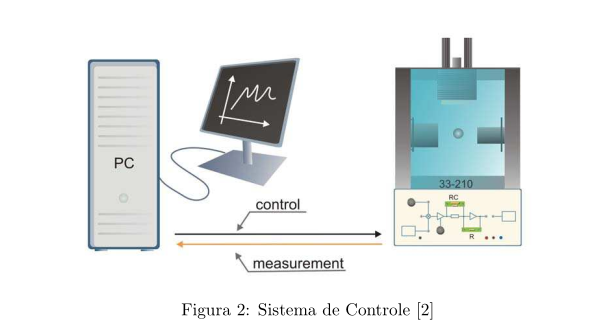
\includegraphics[width=\linewidth]{control.png}
    \caption{ Sistema de Controle [1]}
    \label{fig:2}
\end{figure}
A planta utilizada para estudo é mostrada na Figura 2. O sistema apresentado funciona da seguinte forma:

\begin{itemize}
    \item Um computador, equipado com uma placa de aquisição de dados da Advantech, funciona como unidade central de controle em conjunto com os ambientes MATLAB e Simulink. Os sinais de controle, variando entre -5V e 5V, são enviados ao módulo do levitador, que os converte em corrente elétrica aplicada à bobina, gerando o campo magnético responsável pela levitação.
    \item A posição da esfera magnética é detectada por um senosr infravermelho integrado à estrutura do sistema. Esses dados de posição são transmitidos ao computador por meio da interface de comunicação, onde os algoritmos de controle implementados pelo Simulink processam as informações e ajustam o sistema em tempo real.
\end{itemize}

\subsection{Variáveis do Processo}
\begin{description}
    \item[Variável Manipulada:] Tensão de controle aplicada ao Levitador Magnético.
    \item[Variável Medida:] Posição da esfera, medida pelo sensor infravermelho, convertida em sinal de tensão.
    \item[Variável de Referência:] Posição desejada esfera, set-point. 
\end{description}

\subsection{Sensores e Atuadores}
\begin{description}
    \item[Planta] A unidade mecânica do sistema de levitagão magnética.
    \item[Sensor] Sensor infravermelho usado para medir a posição vertical da esfera suspensa no ar.
    \item[Atuador] Circuito de controle que aplica a tensão ao núcleo magnético, gerando o campo magnético para levitar a esfera. 
\end{description}

\subsection{Pertubações e Não Linearidades}
\begin{description}
    \item[Pertubações] O sistema pode ser afetado por vibrações externas, variações na carga, que podem comprometer a estabilidade da esfera em levitação.
    \item[Não Linearidades] O sistema apresenta característica não linear devido à natureza da força de atração eletromagnética, que pode ser expressa pela seguinte equação: 
    \begin{equation}
        F_{M} = k \frac{i^{2}}{x^{2}}
        \label{eq: forca_magnetica}
    \end{equation}
    em que, $F_{M}$ representa a força magnética, $i$ é a corrente aplicada à bobina, $x$ é a distância vertical da esfera em relação ao sensor, e $k$ é uma constante do sistema.
\end{description}



\section{Especificações de Desempenho Desejado}


\section{Modelagem Matemática}


\section{Identificação por Resposta em Frequência} 


% BIBLIOGRAFIA
\nocite{*}
\bibliography{exemplo}
\cite{mozelli2020}
\cite{oliveira2011}
\cite{parks1999}
\end{document}
